\documentclass{article}
\usepackage[margin=2.5cm]{geometry}
\usepackage{amsmath}
\usepackage{subcaption}
\usepackage{graphicx}

\title{Computing normalization factors for single-cell RNA-seq data: avoiding problems with zero counts}
\author{Aaron Lun and Karsten Bach}

\begin{document}
\maketitle

\section{Introduction}
Single-cell RNA sequencing (scRNA-seq) is a powerful technique that allows researchers to characterize the gene expression profile of single cells.
From each cell, mRNA is isolated, reverse-transcribed and subjected to massively parallel sequencing \cite{stegle2015computational}.
The sequencing reads are then mapped to a reference genome, whereby the number of reads mapped to each gene can be used to quantify the expression of that gene.
Alternatively, transcript molecules can be counted directly using unique molecular identifiers (UMIs) \cite{islam2014quantitative}.
Count data can be analyzed to identify new cell subtypes and to detect highly variable or differentially expressed (DE) genes between cell subpopulations.
This type of single-cell resolution is not possible with bulk RNA sequencing of cellular populations.
However, the downside is that the counts often contain high levels of technical noise with many ``drop-outs'', i.e., zero or near-zero values.
This is due to the difficulties in sequencing low amounts of RNA per cell, which decreases the capture efficiency during library preparation.
Moreover, the capture efficiency often varies from cell to cell, such that counts cannot be directly compared between cells.

Normalization of the scRNA-seq counts is a critical step that corrects for differences in capture efficiency between cells.
Two broad classes of normalization approaches are available -- those using spike-in RNA sets, and those using the counts for cellular RNA.
In the former, the same quantity of spike-in RNA is added to each cell prior to library preparation \cite{stegle2015computational}.
Any difference in the coverage of the spike-in transcripts must be caused by differences in capture efficiency between cells.
Normalization is then performed by scaling the counts to equalize spike-in coverage between cells.
For the methods using the cellular counts, the common assumption is that most genes are not DE across the sampled cells.
Counts are then scaled so that there is, on average, no fold-difference in expression between cells for the majority of genes.
This is the underlying concept of commonly used methods such as size factor \cite{anders2010differential} and trimmed mean of M-values (TMM) normalization \cite{robinson2010scaling}.
An even simpler approach involves scaling the counts to remove differences in library sizes between cells.

The type of normalization that can be used often depends on the characteristics of the data set.
In some data sets, spike-in data may not be present -- for example, droplet-based protocols \cite{klein2015droplet,macosko2015highly} do not allow spike-ins to be easily incorporated.
This obviously precludes the use of spike-in normalization.
The methods based on cellular counts can be applied more generally but have their own deficiencies.
Normalization by library size is insufficient when DE genes are present, as composition biases can introduce spurious differences between cells \cite{robinson2010scaling}.
Size factor or TMM normalization are more robust to DE but rely on the calculation of ratios of counts between cells.
This is not straightforward in scRNA-seq data, where the high frequency of drop-out events interferes with stable normalization.
A large number of zeroes will result in nonsensical size factors or undefined M-values in the TMM method.
One could proceed by removing the offending genes during normalization for each cell, but this may introduce biases if the number of zeroes varies across cells.

Correct normalization of scRNA-seq data is essential as it determines the validity of all downstream quantitative analyses.
In this article, we describe a deconvolution approach that improves the accuracy of the non-DE (i.e., size factor or TMM) normalization methods.
Briefly, normalization is performed on pooled counts for multiple cells, where the incidence of problematic zeroes is reduced
    -- the pooled size/normalization factors are then deconvolved back to those for the individual cells.
Using a variety of simple simulations, we demonstrate that our approach outperforms the direct application of those normalization methods for count data with many zeroes.
We also show a similar difference in behaviour on several real data sets, where deconvolved normalization yields results that are more biologically relevant.
These results suggest that our approach is a viable alternative to existing methods for general normalization of scRNA-seq data.

\section{Existing normalization methods fail with zero counts}

\subsection{The origin of zero counts in scRNA-seq data}
The high frequency of zeroes in scRNA-seq data is driven by both biological and technical aspects.
Gene expression is highly variable across cells due to cell-to-cell heterogeneity and phenomena like transcriptional bursting \cite{marinov2014singlecell}.
Such variability is likely to result in zero counts for the lowly expressed genes.
It is also technically difficult to process low quantities of input RNA into sequenceable libraries.
This results in high dropout rates whereby low-abundance transcripts are not captured during library preparation \cite{brennecke2013accounting}.

It is important to distinguish between stochastic and systematic zeroes.
Systematic zeroes refer to genes that are constitutively silent in a cell (sub)population, such that the count must be zero for all cells in that population.
These are generally not problematic as they contain no information and can be removed prior to normalization.
Stochastic zeroes refer to genes that are actively expressed but obtain counts of zero in some cells due to sampling stochasticity.
It is less clear how to deal with these genes, as they contain information about the relative differences between cells.
Removing them prior to normalization may introduce biases.

\subsection{A brief description of existing non-spike-in methods}
Here, we only consider those normalization methods not based on spike-in data.
This is motivated by the desire to obtain a general method that can be applied in all data sets.
In particular, we will review three approaches that are commonly used for RNA-seq data -- size factor, TMM and library size normalization.

Size factor normalization was originally introduced as part of the DESeq package for differential expression \cite{anders2010differential}.
It first constructs an ``average'' reference library, in which the ``count'' for each gene is defined as the geometric mean of the counts for that gene across all real libraries.
Each real library is then normalized against this average.
Specifically, for each gene, it computes the ratio of the count in each library to that in the average library.
The size factor for each library is defined as the median of this ratio across all genes.
This value represents the extent to which the counts in that library should be downscaled, 
    in order to eliminate any systematic differences in expression between libraries for the majority of (assumed) non-DE genes.

TMM normalization was introduced as part of the edgeR package for differential expression \cite{robinson2010edgeR}.
It selects one library to be a reference, and normalizes each other library against the reference.
Specifically, for each library, M-values (i.e., library size-adjusted log$_2$-ratios in expression) are computed against the reference for all genes.
The genes with the most extreme M-values are trimmed away.
High- or low-abundance genes are similarly removed.
The weighted mean of the remaining M-values is computed, where the weighting is performed according to the asymptotic variance of each M-value.
This is used to define the normalization factor for each library as $2^x$, where $x$ is the weighted mean for that library.
The normalization factor represents the downscaling required to eliminate systematic differences between libraries, additional to that required to equalize the library sizes.
Taking the product of the normalization factor and library size for each library (i.e., the effective library size) yields a value that is functionally equivalent to the size factor.

Both size factor and TMM normalization assume that most genes are not DE between libraries.
Any systematic difference in expression across the majority of genes is treated as bias.
This is duly incorporated into the size/normalization factors and removed upon scaling.
If the non-DE assumption does not hold, the computed factors will not be accurate.
In addition, both methods perform poorly in the presence of a large number of zeroes.
For size factor normalization, the geometric mean is equal to zero for genes with a zero count in any library, such that the ratios for that gene become undefined.
Conversely, a library with zero counts for many genes may have a size factor of zero, which precludes any sensible scaling.
For TMM normalization, M-values are undefined when the count in either library is zero.
In such conditions, both methods typically require \textit{ad hoc} workarounds such as the removal of zero counts within each library.

Finally, library size normalization is another commonly used approach for RNA-seq data.
This involves scaling the counts such that the library size is the same across libraries.
While simple, this approach is not robust in the presence of DE genes \cite{robinson2010scaling}.
One can imagine a scenario where a single gene is strongly upregulated in one library compared to another.
This increases the size of the first library, as more reads are generated from the upregulated gene.
Normalization by library size will then scale up the counts for the second library to compensate.
This introduces spurious differences in the counts between libraries for the non-DE genes.
The likely presence of DE in real data means that library size normalization is often inappropriate.

\subsection{Performance of existing methods on simulated data with zeroes}
To test the performance of existing methods, simulated scRNA-seq data was generated with a large number of stochastic zeros.
For gene $i$ in cell $j$, the count $y_{ij}$ was sampled from a negative binomial (NB) distribution with mean $\theta_{j}\lambda_{i}$.
The $\theta_{j}$ term represents cell-specific biases (e.g., in capture efficiency) that must be normalized out, 
    and is sampled for each cell such that $\log_2(\theta_j) \sim \mathcal{N}(0, 0.25)$.
The $\lambda_{i}$ term denotes the expected number of transcripts for each gene, and is distributed across genes such that $\log_2(\lambda_i) \sim \mbox{Uniform}(3, 6)$.
This recapitulates the spread of abundances in real data.
The NB dispersion is defined for each gene as 
\[
    \varphi_i = 2 + \frac{100}{\lambda_i}
\]
to represent a decreasing mean-dispersion trend.
Large values for $\varphi_i$ are consistent with the high levels of technical noise and biological heterogeneity in scRNA-seq studies,
    and ensure that a large number of stochastic zeroes are generated.
In this manner, counts were generated for 10000 genes across 600 cells.

Size factor and TMM normalization were then applied to this data set.
For size factor normalization, the geometric mean was computed by replacing all zero counts with unity.
Zero counts were also removed within each library prior to calculation of the size factor.
For TMM normalization, all undefined M-values were removed prior to trimming and calculation of the normalization factor for each library.
The corresponding size factor was defined as the effective library size, i.e., the product of the library size and the normalization factor for each library.
Estimated size factors were then compared to the true values $\theta_j$ for all cells.

Figure~\ref{fig:sim_noDE} demonstrates that both methods yield size factors that systematically deviate from the true values.
Large size factors are underestimated while small size factors are overestimated.
This is a consequence of removing stochastic zeroes prior to normalization.
Consider a simple example where a cell with low $\theta_j$ is normalized against a cell with a large $\theta_j$. 
The former cell is likely to contain more stochastic zeroes, as the mean of the sampling distribution for the counts is lower.
Removal of the affected genes will shift the median upwards among the remaining non-zero counts, resulting in overestimates of the size factor.
Similarly, the distribution of M-values will be shifted towards larger values when more zeroes are present in the smaller cell.
This is because zeroes represent sampled values below some non-zero mean, and would generally correspond to negative M-values.
Their removal increases the weighted mean and biases the estimate of the TMM normalization factor.
The converse applies to cells with large $\theta_j$, where a concomitant underestimation is observed in the size factor.
It should be stressed that the non-DE assumption has not been violated in these simulations as all genes are non-DE between cells (other than the systematic biases due to $\theta_j$).
Even under such favourable conditions, the existing methods fail to correctly estimate the size factor for each cell.

\begin{figure}[tb]
\begin{minipage}{0.33\textwidth}
\includegraphics[width=\textwidth]{size_sim_noDE.pdf}
\subcaption{}\label{subfig:size_noDE}
\end{minipage}
\begin{minipage}{0.33\textwidth}
\includegraphics[width=\textwidth]{tmm_sim_noDE.pdf}
\subcaption{}\label{subfig:tmm_noDE}
\end{minipage}
\begin{minipage}{0.33\textwidth}
\includegraphics[width=\textwidth]{sum_sim_noDE.pdf}
\subcaption{}\label{subfig:sum_noDE}
\end{minipage}
\caption{
    Performance of existing normalization methods on the simulated data with stochastic zeroes.
    The size factor estimate for each cell is plotted against its true values for (\subref{subfig:size_noDE}) size factor and (\subref{subfig:tmm_noDE}) TMM normalization.
    Estimates are also shown for our deconvolution approach (\subref{subfig:sum_noDE}).
    Axes are shown on a log-scale for visibility.
    The red line represents equality between the estimated and true factors.
}
\label{fig:sim_noDE}
\end{figure}

\section{Improving normalization accuracy with deconvolution}

\subsection{Description of the algorithm}
Define the size-adjusted expression of gene $i$ as $\pi_{ij} = y_{ij}/T_j$, where $T_j$ is the total library size for cell $j$.
The expectation of $\pi_{ij}$ can then be written as $\theta_j\lambda_i T_j^{-1}$.
Further assume that we have an arbitrary set of cells $\mathcal{S}_k$.
Denote the sum of $\pi_{ij}$ across $\mathcal{S}_k$ as $s_{ik}$ for gene $i$.
The expectation of $s_{ik}$ is equal to 
\[
    E(s_{ik}) = \lambda_i \sum_{j \in \mathcal{S}_k} \theta_j T_j^{-1}\;.
\]
Similarly, define $\mathcal{S}_0$ as the set of all cells in the data set, and $s_{i0}$ as the sum of expression values across all cells for gene $i$.
The expectation of the ratio $r_{ik}$ of the sums between $\mathcal{S}_k$ and $\mathcal{S}_0$ is defined as
\begin{equation}
    E(r_{ik}) \approx \frac{E(s_{ik})}{E(s_{i0})} 
    = \frac{\sum_{\mathcal{S}_k} \theta_j T_j^{-1}}{\sum_{\mathcal{S}_0} \theta_j T_j^{-1}} 
    = \frac{\sum_{\mathcal{S}_k} \theta_j T_j^{-1}}{C}
    \label{eqn:linear_single}
\end{equation}
where $C$ is a constant that does not depend on the gene, cell or set $\mathcal{S}_k$.
The above approximation is valid if the variance of the sums is low, which should be the case for large sets 
    -- the variability relative to the mean should decrease due to the law of large numbers.
This expectation is estimated by taking any robust average (e.g., median) of $r_{ik}$ across $i$.
Robustness protects the average against DE genes with extreme ratios.

The estimated value of $E(r_{ik})$ for the set can be used to obtain estimates for $\theta_j$ for each cell.
A linear equation is set up based on the expression in Equation~\ref{eqn:linear_single}, 
by replacing $E(r_{ik})$ with its estimate and treating the $\theta_j T_j^{-1}$ as unknown parameters to be estimated.
Repeating the estimation of $E(r_{ik})$ for different sets of cells in $\mathcal{S}_{ik}$ will generate a system of linear equations, 
    in which the $\theta_j T_j^{-1}$ for each $j$ is represented at least once.
This system can then be solved to obtain estimates of $\theta_j T_j^{-1}$ for all cells.
Multiplication by $T_j$ for each cell will then yield an estimate of $\theta_j$.
This approach may seem somewhat circuitous, given that $\theta_j$ could be estimated directly from the counts for each cell by itself.
However, summation avoids zeros and near-zero counts that are present in the single-cell data.
These counts are problematic as they interfere with the calculation of median ratios and estimation of $\theta_j$.
Ratios computed from pooled expression profiles are more stable, and this stability will propagate back to the $\theta_j$ estimates when the linear system is solved.

The linear system can be solved using standard methods such as those based on the QR decomposition.
However, with such methods, it is theoretically possible to obtain negative estimates for $\theta_j$.
Such values are obviously nonsensical as counts cannot be scaled to negative values.
The most obvious situation in which this could occur involves samples with very small library sizes relative to the other cells, 
    such that the true value of $\theta_j$ is already close to zero.
Errors in estimation may then be sufficient to push the estimated $\theta_j$ below zero.
In general, this scenario seems somewhat pathological, as samples with abnormally small library sizes should be removed prior to analysis.
Nonetheless, some protection is provided by using linear inverse models \cite{soetaert2009limsolve} to constrain the estimates to non-negative values.
This will not provide sensible estimates for the offending cells -- these are likely to be set to zero, and should be removed prior to further processing --
    but will ensure that the estimates for other cells are not distorted by negative values elsewhere in the system.
    
This approach makes some moderately strong assumptions regarding the nature of DE across the data set.
Consider the summed cells in $\mathcal{S}_k$ and $\mathcal{S}_0$ as a pseudo-cell $k$ and an average reference, respectively.
The use of the median is only valid when less than 50\% of genes are DE in any direction in the pseudo-cell compared to the reference,
    i.e., less than 50\% of genes can be upregulated and less than 50\% of genes can be downregulated.
If more DE genes are present, the median will not represent a robust average across non-DE genes.
This condition generally requires a proportion of genes to be constantly expressed across all cells in the data set 
    -- otherwise, all genes would be DE against the average in at least one pseudo-cell -- 
    and is only guaranteed to be true when that proportion is equal to or greater than 50\% of all genes.
The assumption here is similar to that required for size factor normalization where an average reference is also used.

Note that counts could be summed rather than size-adjusted expression values.
This means that the solution of the linear system will directly yield estimates of $\theta_j$.
However, we use size-adjusted values to ensure that the sum is not dominated by a small number of very large libraries.
Information from each cell will then be weighted equally when computing the median ratio for each set, regardless of library size.

\subsection{Selecting cells to sum}
A key step of this approach lies in how to select cells for each set $\mathcal{S}_{ik}$.
Ideally, one would sum cells with similar expression profiles.
This ensures that the same set of genes are DE against the average for all cells in the set,
    which minimizes the total amount of DE genes in the set and reduces the risk of violating the non-DE assumption.
However, there may not be any prior knowledge regarding the relative similarity of different cells.
This means that dimensionality reduction and clustering would be required to empirically identify groups of similar cells.
Such methods are not straightforward and will be addressed later.

The simpler solution is to use the library size as a rough proxy for cell similarity.
This is motivated by the fact that different cell types tend to have systematic differences in the library sizes, 
    e.g., due to type-specific differences in total RNA or capture efficiency.
First, cells are ordered by their total counts and partitioned into two groups, depending on whether the ranking of each cell is odd or even.
The cells are then arranged in a ring, with odd cells on the left and even cells on the right.
Conceptually, one can start at the 12 o'clock position on the ring, for the largest libraries; moving clockwise through the even cells with decreasing library size;
reaching the smallest libraries at 6 o'clock; and then, continuing to move clockwise through the odd cells with increasing library size (Figure~\ref{fig:library_ring}).
For summation, a sliding window is moved cell-by-cell across this ring.
Each window contains the same number of cells, all of which are of a similar library size.
These cells are used to define a single instance of $\mathcal{S}_{k}$.
Thus, each window defines a separate equation in the linear system.
The use of a ring means that the window is defined at the smallest and largest libraries.
In contrast, sliding a window across a linear ordering of cells will result in truncated windows at the boundaries.

\begin{figure}[bt]
    \begin{center}
        \includegraphics[width=0.5\textwidth]{pics/library_ring.pdf}
    \end{center}
    \caption{
        Ring arrangement of cells ordered by library size.
        Each circle represents a cell where the size of the circle corresponds to the library size of that cell.
        Even- and odd-ranking cells lie on opposite sides, with the largest and smallest libraries at the top and bottom, respectively.
        Cells lying in a window of length 4 are highlighted in red.
        Different instances of the window are obtained by sliding the window across the ring.
    }
    \label{fig:library_ring}
\end{figure}

The total number of equations in the linear system is equal to the number of cells.
The $\theta_j$ term for each cell is represented in $w$ equations, where $w$ denotes the size of the window.
By using different values of $w$, additional equations can be added to improve the precision of the estimates. 
Specifically, values of $w$ are set to 20, 40, 60, 80 and 100.
These are large enough to obtain stable sums yet small enough to maintain resolution, i.e., by ensuring that cells with very different library sizes are not summed together.
This increases the total number of equations in the system and means that each $\theta_j$ is represented in 300 equations. 

An additional set of equations is added to ensure that the system is solvable.
In each equation, the $\theta_j$ for each cell is equated to the size factor estimated directly from its single-cell counts.
These equations are assigned very low weights compared to the other equations involving summed cells, with weights of $10^{-6}$ and unity respectively.
A weighted least-squares approach is then applied to solve the linear system.
In the matrix containing the coefficients of the linear system, the incorporation of the additional equations ensures that the columns are linearly independent.
This ensures that a single solution can be obtained for all $\theta_j$.
Due to their low weights, the additional equations will not contribute substantially to the weighted least-squares solution.
This means that the estimated values are driven primarily by the equations for summed cells.

\subsection{Performance of the deconvolution approach}
We will refer to the approach described above as the deconvolution method, as it deconvolves the size factors for each cell from the size factors of the sum.
Application of the deconvolution method to the simulated data yields accurate estimates of the size factors (Figure~\ref{subfig:sum_noDE}).
This is consistent with the reduced number of zero counts in the summed counts for each set of cells.
The median ratio for each set is more accurately computed, which improves the accuracy of the size factor estimates for the individual cells upon deconvolution.
Systematic under- or overestimation of the size factors for cells with large or small $\theta_j$ is avoided.

\section{Robustness to violations of the non-DE assumption}

\subsection{All methods fail without a non-DE majority}
The performance of each method was evaluated on simulated data with DE genes.
In the simulation design described above, the 600 cells were partitioned into three subpopulations of 200 cells.
In subpopulation $s=1$, 3000 genes were randomly chosen and the expected number of transcripts $\lambda_{is}$ for gene $i$ was set to $2\lambda_{i}$.
This was repeated with a different set of 3000 genes for subpopulation $s=2$ with $\lambda_{is}=4\lambda_i$; and again in the last subpopulation $s=3$, with $\lambda_{is}=6\lambda_i$.
Each set of upregulated genes represents the unique expression signature for the corresponding subpopulation.
The value of $\theta_j$ for each cell was sampled as previously described, independently of the subpopulation of that cell.
The count for each gene in each cell was then sampled from a NB distribution with a mean of $\theta_j\lambda_{is}$ for all signature genes and $\theta_j\lambda_i$ otherwise.

% The use of a different fold-increase for each subpopulation is necessary, otherwise the average expression profile is flat, which is unlikely for real data.

All methods failed to accurately estimate the true $\theta_j$ in this simulation (Figure~\ref{fig:sim_DE}).
This is consistent with the violation of the non-DE assumption.
Across the three subpopulations, there are 9000 genes involved in subpopulation-specific signatures, i.e., 90\% of all genes exhibit DE within this data set.
An assumption of a non-DE majority of genes is clearly invalid in this scenario.
Any systematic differences in expression between cells of different subpopulations will now include genuine DE in addition to cell-specific biases.
Subsequently, the magnitude of DE will be incorporated in the size factors computed from each method, such that they are no longer accurate estimates of $\theta_j$.
The estimates also split into two distinct groups within each plot of Figure~\ref{fig:sim_DE}.
The lower group corresponds to the first subpopulation which has the weakest expression signature in this simulation (2-fold upregulation).
Size factors for cells in this subpopulation are underestimated as strong DE in the signature genes of other subpopulations drags down the median ratio/trimmed mean.

\begin{figure}[tb]
\begin{minipage}{0.33\textwidth}
\includegraphics[width=\textwidth]{size_sim_DE.pdf}
\subcaption{}\label{subfig:size_DE}
\end{minipage}
\begin{minipage}{0.33\textwidth}
\includegraphics[width=\textwidth]{tmm_sim_DE.pdf}
\subcaption{}\label{subfig:tmm_DE}
\end{minipage}
\begin{minipage}{0.33\textwidth}
\includegraphics[width=\textwidth]{sum_sim_DE.pdf}
\subcaption{}\label{subfig:sum_DE}
\end{minipage}
\caption{
    Performance of existing normalization methods on simulated data with subpopulation-specific DE genes and stochastic zeroes.
    The size factor estimate for each cell is plotted against its true values for (\subref{subfig:size_noDE}) size factor and (\subref{subfig:tmm_noDE}) TMM normalization.
    Estimates are also shown for our deconvolution approach (\subref{subfig:sum_noDE}).
    Cells in the first, second and third subpopulations are shown in black, blue and orange, respectively.
    Axes are shown on a log-scale for visibility.
    The red line represents equality between the estimated and true factors.
}
\label{fig:sim_DE}
\end{figure}

It is worth noting that the partition between subpopulations is clearer for the deconvolution method compared to the existing methods.
This is due to the presence of stochastic zeroes, which are responsible for the systematic over- and under-estimation of small and large $\theta_j$ in the existing methods.
As a result, the estimates for different subpopulations are squeezed together in Figures~\ref{subfig:size_DE} and \ref{subfig:tmm_DE}.
The deconvolution method avoids these problems, leading to a sharper distinction between subpopulations in Figure~\ref{subfig:sum_DE}. 
Obviously, however, the greater issue of inaccuracy in the presence of DE genes is not resolved by deconvolution.

\subsection{Improving accuracy with clustering prior to normalization}

\section{Something something real data}

\bibliographystyle{unsrt}
\bibliography{references}

\end{document}

